\documentclass[10pt]{article}
% TMLR style (github.com/JmlrOrg/tmlr-style-file, commit 7bf90ef, Apache-2.0).
% Submission: anonymous. Preprint: [preprint]. Camera-ready: [accepted].
\usepackage[preprint]{tmlr}
\usepackage[T1]{fontenc}
\usepackage{amsmath,amssymb,amsthm}
\usepackage{booktabs}
\usepackage{graphicx}
\usepackage{xcolor}
\usepackage[hidelinks]{hyperref}
\usepackage{caption}
\captionsetup{font=small}
\newtheorem{proposition}{Proposition}

% Every number below that comes from data is a macro written by
% chemistry_elevation/scripts/make_figures.py from stored artifacts.
% Generated by chemistry_elevation/scripts/make_figures.py. Do not edit.
\newcommand{\valaAlpha}{8.1}
\newcommand{\valaBias}{0.050}
\newcommand{\valaCI}{0.048}
\newcommand{\valaCov}{10}
\newcommand{\valaESS}{79}
\newcommand{\valaErr}{0.122}
\newcommand{\valaFexact}{-3.392}
\newcommand{\valaGfwd}{0.028}
\newcommand{\valaGrev}{11.7}
\newcommand{\valaSamp}{<0.01}
\newcommand{\vbdBidir}{6.8}
\newcommand{\vbdCov}{0}
\newcommand{\vbdCovMin}{0}
\newcommand{\vbdESS}{98}
\newcommand{\vbdESSMin}{0}
\newcommand{\vbdEps}{10^{-6}}
\newcommand{\vbdErr}{0.69}
\newcommand{\vbdJensen}{0.009}
\newcommand{\vbdM}{1{,}000}
\newcommand{\vbdNoDisc}{99.8}
\newcommand{\vbdRuns}{400}
\newcommand{\vbdTarget}{0.69}
\newcommand{\vchigBias}{0.010}
\newcommand{\vchigBiasHi}{0.021}
\newcommand{\vchigBiasLo}{0.002}
\newcommand{\vchigBlockMax}{7}
\newcommand{\vchigBlockMin}{0}
\newcommand{\vchigFirstFifth}{6.3}
\newcommand{\vchigFrames}{30{,}000}
\newcommand{\vchigLastHalf}{0.3}
\newcommand{\vchigLitBias}{0.68}
\newcommand{\vchigLitNative}{68}
\newcommand{\vchigMinRMSD}{1.20}
\newcommand{\vchigNative}{1.7}
\newcommand{\vchigNativeHi}{3.4}
\newcommand{\vchigNativeLo}{0.3}
\newcommand{\vcovDiffOneFive}{60}
\newcommand{\vcovDiffTwo}{8}
\newcommand{\vcovDiffZeroSix}{94}
\newcommand{\vcovGFNOneFive}{71}
\newcommand{\vcovGFNTwo}{47}
\newcommand{\vcovGFNZeroSix}{94}
\newcommand{\vcovPAOneFive}{96}
\newcommand{\vcovPATwo}{95}
\newcommand{\vcovPAZeroSix}{96}
\newcommand{\vcovVANOneFive}{96}
\newcommand{\vcovVANTwo}{92}
\newcommand{\vcovVANZeroSix}{95}
\newcommand{\verrDiffOneFive}{1.3\times10^{-2}}
\newcommand{\verrGFNOneFive}{2.4\times10^{-2}}
\newcommand{\verrPAOneFive}{7.8\times10^{-4}}
\newcommand{\verrSATIOneFive}{7.1\times10^{-4}}
\newcommand{\verrVANOneFive}{8.6\times10^{-5}}
\newcommand{\vinstClassical}{200}
\newcommand{\vinstLearnedMax}{30}
\newcommand{\vinstLearnedMin}{20}
\newcommand{\vljEfcc}{-173.928}
\newcommand{\vljEico}{-173.252}
\newcommand{\vljLitIco}{90}
\newcommand{\vljNT}{7}
\newcommand{\vljPfccMin}{100}
\newcommand{\vljTmax}{0.18}
\newcommand{\vljTmin}{0.06}
\newcommand{\vsecDiff}{6.96}
\newcommand{\vsecGFN}{30.60}
\newcommand{\vsecPA}{0.08}
\newcommand{\vsecSATI}{0.06}
\newcommand{\vsecVAN}{2.49}
\newcommand{\vtoyMassOne}{50.1}
\newcommand{\vtoyMassTwo}{49.9}
\newcommand{\vtoySplit}{-0.54}
\newcommand{\vtoyZone}{5.88}
\newcommand{\vtoyZtwo}{5.85}
\newcommand{\vtrpBias}{0.417}
\newcommand{\vtrpBiasHi}{0.501}
\newcommand{\vtrpBiasLo}{0.335}
\newcommand{\vtrpBlockMax}{64}
\newcommand{\vtrpBlockMin}{24}
\newcommand{\vtrpFirstFifth}{53.0}
\newcommand{\vtrpFrames}{30{,}000}
\newcommand{\vtrpLastHalf}{55.1}
\newcommand{\vtrpLitBias}{1.02}
\newcommand{\vtrpLitNative}{82}
\newcommand{\vtrpMinRMSD}{0.50}
\newcommand{\vtrpNative}{50.3}
\newcommand{\vtrpNativeHi}{56.8}
\newcommand{\vtrpNativeLo}{43.0}
\newcommand{\vvanOverSati}{8}


\newcommand{\E}{\mathbb{E}}
\newcommand{\ESS}{\mathrm{ESS}}
\title{False Confidence in Generative Samplers:\\Exact Physical References Expose Hidden Errors and Diagnostic Blindness}
% Hidden by tmlr.sty in submission mode; printed with [preprint] or [accepted].
\author{\name Karthik Gangadharaiah \\
      \addr Independent researcher (KoWerk), Amsterdam, The Netherlands \\
      ORCID: \href{https://orcid.org/0009-0009-1713-8624}{0009-0009-1713-8624}}
\def\month{MM}
\def\year{YYYY}
\def\openreview{\url{https://openreview.net/forum?id=XXXX}}

\begin{document}
\maketitle

\begin{abstract}
Learned samplers are increasingly proposed for equilibrium sampling and free energies in chemistry, and they are usually judged by self-normalized diagnostics such as the effective sample size (ESS). We show with an elementary proposition that these diagnostics are structurally invariant to the Boltzmann mass $\alpha$ of unvisited basins: conditioned on not proposing a basin, the importance weights follow the law of the truncated system, so the ESS stays high while the free energy shifts by $-k_BT\log(1-\alpha)$ and the nominal delta-method interval contracts around the biased value, yielding asymptotically zero coverage. In a toy double well where one basin holds $\vtoyMassTwo\%$ of the mass, a proposal putting mass $\vbdEps$ on that basin achieves a median ESS of $\vbdESS\%$ but covers the exact $\log Z$ in $\vbdCov\%$ of $\vbdRuns$ runs. On exactly enumerated Sherrington-Kirkpatrick instances ($n=24$), nominal 95\% intervals from masked diffusion and a GFlowNet cover the truth in only $\vcovDiffTwo\%$ and $\vcovGFNTwo\%$ of runs at $\beta=2$, while classical estimators and an autoregressive network (VAN-MADE) stay near 95\%. A reverse check that scores the proposal on draws from an independent reference sampler flags the dropped basin where the forward Jensen gap is blind. We demonstrate this on a continuous molecular model: a RealNVP Boltzmann generator trained on the alanine dipeptide Ramachandran landscape drops the $C_{7\rm ax}$ basin ($\valaAlpha\%$ mass), reporting a median ESS of $\valaESS\%$ with only $\valaCov\%$ coverage, while the reverse check detects the omission ($G_{\rm rev} = \valaGrev$\,nats). Finally, we size the bound on macromolecular systems (chignolin, Trp-cage, LJ$_{38}$), contrasting single-trajectory kinetic trapping with converged Anton and NMR equilibrium baselines to show that dropped macroscopic states shift free energies by $\vchigLitBias$ to $\vtrpLitBias$\,kcal/mol, exceeding lead-optimization thresholds.
\end{abstract}

\section{Introduction}
\label{sec:intro}
Normalizing flows, diffusion models and generative flow networks (GFlowNets) are proposed as samplers of Boltzmann distributions $p(x)\propto e^{-\beta U(x)}$ for molecules and materials \citep{noe2019boltzmann,hoogeboom2022edm,satorras2021egnn,lipman2023flowmatching}. The partition function $Z$ of such systems is unknown, so a learned sampler is usually judged by statistics of its own importance weights: the effective sample size (ESS), the Pareto $\hat k$, and delta-method intervals for the free energy.

These statistics share a critical failure mode: they are computed exclusively from configurations the sampler proposed, so a basin it never proposes leaves no trace in them. Section~\ref{sec:theory} formalizes this diagnostic blindness: conditioned on never visiting a basin of Boltzmann mass $\alpha$, the importance weights follow the law of the problem with that basin deleted. As a result, the free-energy estimate is shifted by $-\beta^{-1}\log(1-\alpha)$ while the ESS remains high and nominal confidence intervals shrink at rate $O(M^{-1/2})$ around the wrong value, so coverage falls toward 0\% for as long as the basin stays unvisited (Figure~\ref{fig:molecular_pathology}). While support coverage is an elementary requirement of importance sampling, modern evaluation culture has overlooked a critical consequence: self-reported diagnostics falsely reward mode collapse with high confidence, reporting near-optimal ESS and contracting intervals precisely when macroscopic states are omitted.

\begin{figure}[t]
\centering
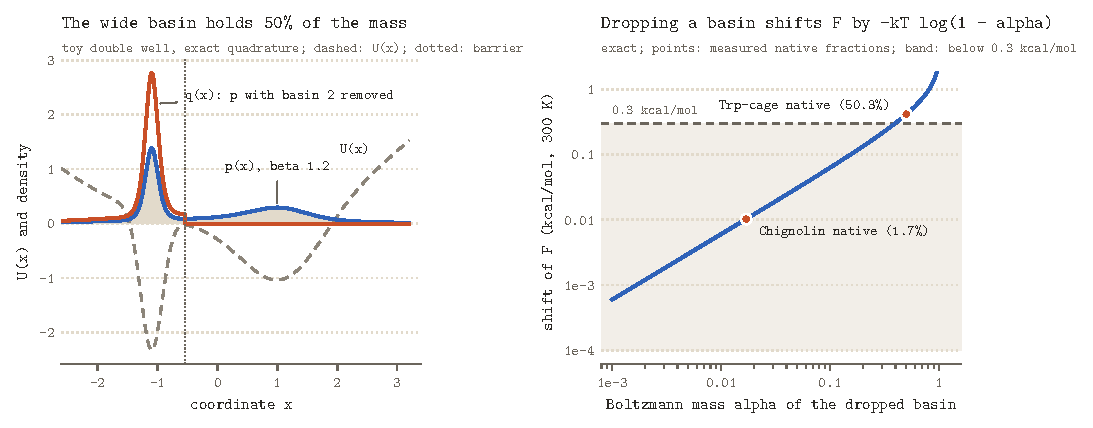
\includegraphics[width=\linewidth]{figures/fig_molecular_pathology.pdf}
\caption{Left: the toy double well of Section~\ref{sec:bidirectional} at $\beta=1.2$. The narrow basin is the energy minimum, but the wide basin holds $\vtoyMassTwo\%$ of the Boltzmann mass (exact quadrature). Shaded: $p$. $q$ is $p$ with the wide basin removed. Right: shift of the free energy at 300\,K when a basin of mass $\alpha$ is never proposed, $-k_BT\log(1-\alpha)$ (exact). Points mark native-basin fractions; shaded: shifts below 0.3\,kcal/mol.}
\label{fig:molecular_pathology}
\end{figure}

To determine how this pathology manifests across physical systems, we organize our evaluation into three tiers:
\begin{enumerate}
\item \textbf{Exact empirical audit on disordered systems (Section~\ref{sec:benchmarks}):} Spin glasses feature frustrated, multi-basin landscapes where ground-truth partition functions can be enumerated exactly up to $n=28$ spins. On these references, masked diffusion and GFlowNets exhibit severe calibration collapse, covering exact values in only $\vcovDiffTwo\%$ and $\vcovGFNTwo\%$ of runs at $\beta=2$. In contrast, classical thermal estimators and normalized autoregressive networks (VAN-MADE) remain calibrated near 95\%.
\item \textbf{Continuous neural molecular sampler (Section~\ref{sec:bidirectional}):} On an analytic surrogate of the alanine dipeptide Ramachandran surface, a RealNVP flow trained by reverse KL drops the $C_{7\rm ax}$ basin ($\valaAlpha\%$ mass), yet reports a median ESS of $\valaESS\%$ while nominal interval coverage collapses to $\valaCov\%$. An independent reverse check immediately flags the omission ($G_{\rm rev} = \valaGrev$\,nats).
\item \textbf{Macromolecular landscape sizing (Section~\ref{sec:molecular_case}):} We size the bound in kcal/mol with all-atom simulations of chignolin and Trp-cage and a Langevin sweep of the LJ$_{38}$ cluster. Omitting the Trp-cage native basin would shift $F$ by $\vtrpBias$\,kcal/mol at the fraction measured in our run; single trajectories also show the blind spot themselves, since they report nothing about basins they have not reached.
\end{enumerate}

\paragraph{Contributions.} (i) A formal proposition proving that self-normalized diagnostics and confidence intervals are blind to unvisited Boltzmann mass (Section~\ref{sec:theory}). (ii) A combinatorial benchmark comparing learned versus classical samplers against exact ground truth (Section~\ref{sec:benchmarks}). (iii) A reverse check that flags dropped basins in an exact toy and in flows on model landscapes, with its limits (Section~\ref{sec:bidirectional}). (iv) Molecular simulations that size the shift in kcal/mol and show the single-trajectory analogue (Section~\ref{sec:molecular_case}).

\section{Related work}
\label{sec:related}
\paragraph{Neural samplers.} Variational autoregressive networks \citep{wu2019van} and Boltzmann generators \citep{noe2019boltzmann} introduced learned samplers for physical systems. Later work uses equivariant diffusion \citep{hoogeboom2022edm,satorras2021egnn}, flow matching \citep{lipman2023flowmatching,albergo2023building,bose2023se3flow}, discrete diffusion \citep{austin2021d3pm,zhu2025mdns,du2026metadns}, annealed transport \citep{holderrieth2025leaps} and GFlowNets \citep{bengio2021gfn,malkin2022tb}.

\paragraph{Free-energy estimators.} Bennett's acceptance ratio \citep{bennett1976bar} and its multistate form \citep{shirts2008mbar} combine forward and reverse samples, and the Jarzynski and Crooks relations \citep{jarzynski1997nonequilibrium,crooks1999entropy} connect nonequilibrium work to free energies. The reverse check of Section~\ref{sec:bidirectional} uses the same two-sided idea. \citet{xu2026modecollapse} proposes a ground-truth-free check for mode collapse, and \citet{fu2023forces} shows that force accuracy does not guarantee correct simulations for learned force fields.

\paragraph{Spin glasses.} The Sherrington-Kirkpatrick (SK) model \citep{sk1975} has a frustrated landscape whose free energy in the limit $n\to\infty$ is given by the Parisi formula \citep{parisi1980}, proven by \citet{guerra2003} and \citet{talagrand2006}. For small $n$ the partition function is computed exactly by enumeration.


\section{Unvisited support}
\label{sec:theory}
Let $(\Omega, \mathcal{F}, \mu)$ be a configuration space endowed with a dominating reference measure $\mu$ (Lebesgue measure for continuous coordinates, counting measure for discrete spins). Let $U: \Omega \to \mathbb{R}$ be a measurable potential energy and $p(x)=e^{-\beta U(x)}/Z$ the Boltzmann probability density with respect to $\mu$, with partition function $Z = \int_\Omega e^{-\beta U(x)}\,d\mu(x)$ and free energy $F=-\beta^{-1}\log Z$. A learned proposal density $q_\theta$ (with $q_\theta(x) > 0$ for $\mu$-almost all $x$ where $p(x) > 0$) is trained to approximate $p$, for example by minimizing $\mathrm{KL}(q_\theta\,\|\,p)$ \citep{noe2019boltzmann}. Given i.i.d.\ draws $x_1,\dots,x_M\sim q_\theta$, the importance-sampling estimate is
\begin{equation}
w_k=\frac{e^{-\beta U(x_k)}}{q_\theta(x_k)},\qquad \hat Z_M=\frac1M\sum_{k=1}^M w_k,\qquad \hat F_M=-\beta^{-1}\log\hat Z_M,
\end{equation}
its reliability is judged by the self-normalized effective sample size
\begin{equation}
\ESS_M=\frac{\left(\sum_k w_k\right)^2}{\sum_k w_k^2},
\end{equation}
and a nominal 95\% interval is $\hat F_M\pm1.96\,\beta^{-1}\hat\sigma_w/(\sqrt M\,\hat Z_M)$, where $\hat\sigma_w$ is the sample standard deviation of the weights.

\begin{proposition}[Diagnostic blindness under unvisited support]
\label{prop:unvisited}
Let $A, B \in \mathcal{F}$ form a measurable partition of $\Omega$ ($A \cap B = \emptyset$, $A \cup B = \Omega$) with $p(B)=\alpha \in (0, 1)$ and $q_\theta(B)=\epsilon \in [0, 1)$. Let $\mathcal E$ be the event that no draw lands in $B$ (all $M$ draws land in $A$). Then
\begin{enumerate}
\item $\mathbb P(\mathcal E)=(1-\epsilon)^M$, which tends to 1 as $\epsilon\to0$ for fixed $M$;
\item conditioned on $\mathcal E$, the draws are conditionally i.i.d.\ with density $q_A(x)=q_\theta(x)\mathbf{1}_A(x)/(1-\epsilon)$;
\item conditioned on $\mathcal E$, $\E[\hat Z_M\mid\mathcal E]=(1-\alpha)Z/(1-\epsilon)$, and by continuous mapping $\hat F_M \xrightarrow{p} F-\beta^{-1}\log\frac{1-\alpha}{1-\epsilon}$ as $M \to \infty$, which approaches $F-\beta^{-1}\log(1-\alpha)$ when $\epsilon \ll \alpha$;
\item conditioned on $\mathcal E$, the joint law of the normalized weights $\tilde{w}_k = w_k/\sum_jw_j$, and hence of $\ESS_M$ and of the relative interval width $\hat\sigma_w/\hat Z_M$, depends on $p$ and $q_\theta$ solely through their conditional restrictions on $A$, and is strictly invariant to $\alpha$ and to the potential landscape on $B$, provided $U$ on $A$ is held fixed.
\end{enumerate}
\end{proposition}

\begin{proof}
Because the draws $x_k$ are i.i.d., $\mathbb P(\mathcal E)=\prod_{k=1}^M \mathbb P(x_k\in A)=(1-\epsilon)^M$. Conditioned on the product event $\mathcal E$, each draw has conditional density $q_\theta(x\mid x \in A)=q_A(x)$ independently. For $x\in A$,
\begin{equation}
\E_{q_A}[w]=\int_A\frac{e^{-\beta U(x)}}{q_\theta(x)}\,\frac{q_\theta(x)}{1-\epsilon}\,d\mu(x)=\frac{Z_A}{1-\epsilon},\qquad Z_A=\int_Ae^{-\beta U(x)}d\mu(x)=(1-\alpha)Z.
\end{equation}
By the weak law of large numbers conditioned on $\mathcal{E}$, $\hat{Z}_M \xrightarrow{p} (1-\alpha)Z/(1-\epsilon)$. Since $g(z) = -\beta^{-1}\log z$ is continuous on $(0, \infty)$, the continuous mapping theorem yields $\hat{F}_M \xrightarrow{p} F - \beta^{-1}\log\frac{1-\alpha}{1-\epsilon}$, proving item 3. For item 4, write $e^{-\beta U(x)}=Z_A\,p(x\mid A)$ for $x \in A$. Then $w_k=c\,p(x_k\mid A)/q_A(x_k)$ where $c=Z_A/(1-\epsilon)$ is a positive scaling constant. The normalized weights $\tilde{w}_k = w_k/\sum_j w_j = \frac{p(x_k\mid A)/q_A(x_k)}{\sum_j p(x_j\mid A)/q_A(x_j)}$ cancel $c$ identically, so their joint distribution depends on $p$ and $q_\theta$ solely through their restrictions to $A$. Changing $\alpha$ or altering $U$ on $B$ while preserving $U|_A$ only shifts $c$, leaving the joint law of the normalized weights, $\ESS_M$, and $\hat\sigma_w/\hat Z_M$ strictly unchanged.
\end{proof}

\paragraph{Diagnostic consequence: coverage collapse.}
The practical danger is not merely that importance sampling requires support coverage: it is the structural blindness of self-reported metrics. By item 4, if a model places negligible mass $\epsilon \ll 1/M$ on a basin, the event $\mathcal E$ occurs with high probability ($>99.9\%$ for $\epsilon=10^{-6}$, $M=10^3$). Conditioned on $\mathcal E$, the sample variance $\hat\sigma_w^2$ and tail diagnostics such as Pareto $\hat{k}$ \citep{vehtari2024psis} reflect only the fit within $A$. In any regime where $\epsilon \ll 1/M$ as sample size $M$ grows, the nominal delta-method confidence interval contracts at rate $O(M^{-1/2})$ around the biased target $F-\beta^{-1}\log(1-\alpha)$, while $\ESS_M/M$ can approach 100\% and $\hat{k}$ remains falsely reassuring ($<0.5$). Consequently, the empirical coverage of the nominal 95\% interval collapses asymptotically to 0\%.

In continuous state spaces, $A$ and $B$ are Borel measurable sets, and $q_A(x) = q_\theta(x)/\int_A q_\theta$ is well-defined whenever $q_\theta(x) > 0$ on $A$. While continuous neural proposals typically have non-zero support everywhere due to diffuse Gaussian tails, this pathology remains operant whenever a physical basin is separated by high free-energy barriers or entropic bottlenecks. If the proposal assigns probability $\epsilon \ll 1/M$ to that basin, no finite sample will visit it, leaving the empirical weights truncated and the diagnostics blind.

The right panel of Figure~\ref{fig:molecular_pathology} illustrates the scale of this bias: at 300\,K a dropped basin must hold about $\vtrpNative\%$ of the mass (as Trp-cage does in our trajectory) to shift $F$ by $\vtrpBias$\,kcal/mol, exceeding common chemical accuracy targets, while a basin holding $\vchigNative\%$ (chignolin in our trajectory) shifts $F$ by only $\vchigBias$\,kcal/mol. Related failure modes for mode-collapsed discrete samplers were observed by \citet{xu2026modecollapse}.

\section{Why spin glasses are a fair test}
\label{sec:isomorphism}
A natural objection is that discrete Ising spins on a complete graph are physically distinct from continuous molecular conformations in three dimensions. The mathematical statement of Proposition~\ref{prop:unvisited} is coordinate-free: it requires only that the target distribution possess multiple metastable basins separated by barriers, and that the proposal fails to populate at least one of them. What an empirical benchmark requires is a system with many such frustrated basins where the true partition function is known exactly, without relying on approximate reference simulations.

The Sherrington-Kirkpatrick (SK) model, $H_n(\sigma)=n^{-1/2}\sum_{i<j}g_{ij}\sigma_i\sigma_j$ with $g_{ij}\sim\mathcal N(0,1)$, provides exactly this setting. Below the critical temperature ($\beta > 1$), its free-energy landscape fractures into a hierarchical ultrametric tree of pure states with extensive Hamming barriers \citep{parisi1980,talagrand2006}. For $n\le28$ spins ($2^{28}\approx 2.68\times 10^8$ configurations), the complete state space can be enumerated exactly (a Gray-code enumerator in Rust in the companion benchmark), yielding exact partition functions and Boltzmann weights.

We do not claim that mean-field spin glasses replicate the Euclidean geometry, bond constraints, or continuous transition paths of atomistic proteins. The role of the SK model is a rigorous falsification test: if an architecture or diagnostic cannot reliably detect the omission of macroscopic states in an exactly-solvable system with known truth, it provides no mathematical or empirical justification for confidence on continuous molecular landscapes where ground truth is unknown.

\section{Exact audit on spin glasses}
\label{sec:benchmarks}
We evaluate the main test split of the SpinGlassBench benchmark at $n=24$: Gaussian SK instances, seven inverse temperatures $\beta\in\{0.3,0.6,0.9,1,1.2,1.5,2\}$, an equal budget of $10^5$ energy evaluations per estimate across all methods, exact $\log Z$ from Gray-code enumeration, and 5 seeds per instance. Classical estimators were evaluated across $\vinstClassical$ instances ($1{,}000$ runs total); computationally intensive learned methods were trained and evaluated across $\vinstLearnedMin$ to $\vinstLearnedMax$ instances ($100$ to $150$ runs total). Table~\ref{tab:chemical_audit} and Figure~\ref{fig:audit_comparison} report summary metrics from this benchmark.

\begin{table}[t]
\centering\small
\caption{SK, $n=24$, test split, $10^5$ energy evaluations per estimate, 5 seeds per instance. Error: mean $|\log\hat Z-\log Z|/n$. Coverage: share of nominal 95\% intervals containing exact $\log Z$ (Clopper-Pearson 95\% binomial CIs in text); n/a: method reports no interval. Seconds: mean wall-clock per estimate at $\beta=1.5$, one thread; learned methods include training.}
\label{tab:chemical_audit}
\begin{tabular}{lrrrrr}
\toprule
Method & \multicolumn{2}{c}{$|\log\hat Z-\log Z|/n$} & \multicolumn{2}{c}{Coverage (\%)} & Seconds \\
\cmidrule(lr){2-3}\cmidrule(lr){4-5}
 & $\beta=0.6$ & $\beta=1.5$ & $\beta=0.6$ & $\beta=1.5$ & per estimate \\
\midrule
SA-TI & $2.4\times10^{-4}$ & $7.1\times10^{-4}$ & n/a & n/a & 0.06 \\
PT-TI & $2.8\times10^{-4}$ & $8.7\times10^{-4}$ & n/a & n/a & 0.11 \\
AIS & $2.7\times10^{-4}$ & $8.9\times10^{-4}$ & 96 & 94 & 0.07 \\
SMC & $2.7\times10^{-4}$ & $8.8\times10^{-4}$ & 96 & 95 & 0.07 \\
PA & $2.7\times10^{-4}$ & $7.8\times10^{-4}$ & 96 & 96 & 0.08 \\
\midrule
VAN-MADE & $2.7\times10^{-5}$ & $8.6\times10^{-5}$ & 95 & 96 & 2.49 \\
Masked diffusion & $1.6\times10^{-4}$ & $1.3\times10^{-2}$ & 94 & 60 & 6.96 \\
GFlowNet & $1.5\times10^{-3}$ & $2.4\times10^{-2}$ & 94 & 71 & 30.60 \\
\bottomrule
\end{tabular}

\end{table}

\begin{figure}[t]
\centering
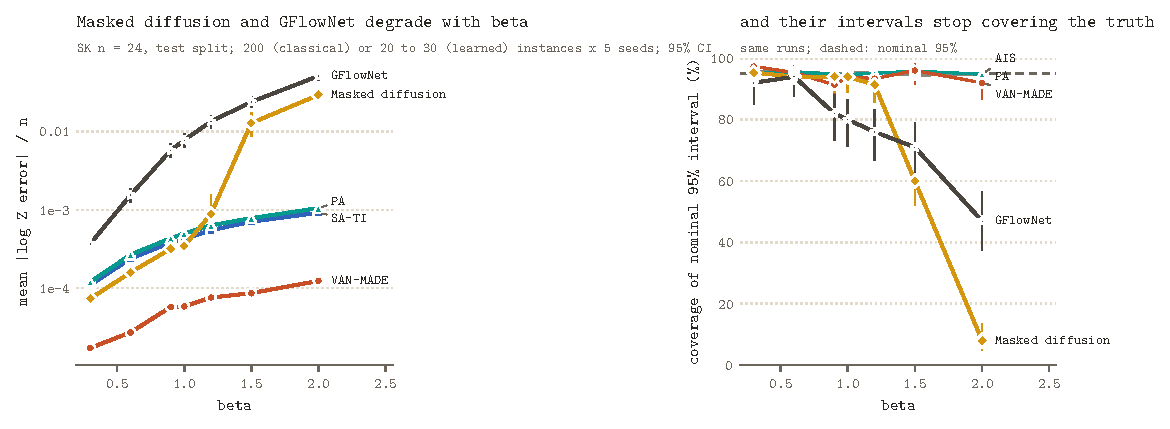
\includegraphics[width=\linewidth]{figures/fig_audit_comparison.pdf}
\caption{Left: mean absolute error of $\log Z$ per spin against $\beta$. Right: coverage of nominal 95\% intervals. SK $n=24$, test split, 5 seeds per instance; error bars are 95\% intervals over instances. Dashed: nominal 95\%.}
\label{fig:audit_comparison}
\end{figure}

\paragraph{Accuracy and architectural divergence.} At $\beta=1.5$, error per spin is $\verrSATIOneFive$ for simulated annealing with thermodynamic integration (SA-TI) and $\verrPAOneFive$ for population annealing (PA). Crucially, learned samplers show sharp architectural divergence:
\begin{itemize}
\item \textbf{Normalized autoregressive networks (VAN-MADE):} Achieve the highest accuracy per energy evaluation ($\verrVANOneFive$, roughly $\vvanOverSati$ times lower error than SA-TI) and maintain calibrated coverage across all temperatures: $\vcovVANZeroSix\%$ at $\beta=0.6$ ($\vcovNVANZeroSix$ runs; 95\% Clopper-Pearson interval $\vcovCIVANZeroSix$), $\vcovVANOneFive\%$ at $\beta=1.5$ ($\vcovCIVANOneFive$), and $\vcovVANTwo\%$ at $\beta=2$ ($\vcovCIVANTwo$), close to PA at $\beta=2$ ($\vcovPATwo\%$, $\vcovNPATwo$ runs, $\vcovCIPATwo$). A possible reason, which we have not tested, is that an autoregressive model's exactly normalized probabilities make the reverse-KL gradient sensitive to missing mass. However, this relies on a 1D sequence factorization ($p(\sigma)=\prod_i p(\sigma_i\mid\sigma_{<i})$). In continuous 3D molecular coordinates, autoregressive factorizations over all atom positions are geometrically constrained and break Euclidean equivariance, which is one reason diffusion models and continuous flows are more common in chemistry.
\item \textbf{Iterative generative samplers (Masked Diffusion and GFlowNets):} Are one to two orders of magnitude less accurate ($\verrDiffOneFive$ and $\verrGFNOneFive$) and undergo catastrophic calibration collapse in the spin-glass phase ($\beta \ge 1.5$). Masked diffusion coverage falls from $\vcovDiffZeroSix\%$ ($\vcovCIDiffZeroSix$) at $\beta=0.6$ to $\vcovDiffOneFive\%$ ($\vcovCIDiffOneFive$) at $\beta=1.5$ and $\vcovDiffTwo\%$ ($\vcovNDiffTwo$ runs, $\vcovCIDiffTwo$) at $\beta=2$. GFlowNet coverage drops to $\vcovGFNOneFive\%$ ($\vcovCIGFNOneFive$) and $\vcovGFNTwo\%$ ($\vcovNGFNTwo$ runs, $\vcovCIGFNTwo$).
\end{itemize}
On one test instance, illustrated in the companion paper, the diffusion sampler keeps one side of the overlap distribution and the GFlowNet concentrates on a few overlaps. By Proposition~\ref{prop:unvisited}, this omitted mass does not widen nominal intervals, producing false confidence.

\paragraph{Wall-clock trade-offs.} Table~\ref{tab:chemical_audit} reports single-thread CPU execution time, with learned methods including training. Under this metric, SA-TI finishes in $\vsecSATI$\,s and PA in $\vsecPA$\,s, whereas VAN-MADE requires $\vsecVAN$\,s and diffusion requires $\vsecDiff$\,s. While neural samplers can amortize training costs when millions of samples are required, on single-target free-energy evaluations classical annealing remains substantially faster.

\paragraph{External code audits.} The companion SpinGlassBench study used the same exact references to score released checkpoints of published samplers; we summarize its results. In MDNS \citep{zhu2025mdns}, the released free-energy estimator rounds one per-step term in bfloat16, which biases $\log Z$ upward by up to $4.6\times10^{-4}$ per site; a one-line change removes the bias. MetaDNS \citep{du2026metadns}, which shares this code, is unbiased at its float16 default. In LEAPS \citep{holderrieth2025leaps}, free energies at the released time grids are low by $2.2$ to $3.2\times10^{-3}$ per site, mostly from time discretization. The ESS did not reveal these errors: for MDNS the biased and corrected estimators have nearly the same ESS, and for LEAPS the ESS fraction is 0.82 on Ising (biased) and 0.31 on Potts, where it is no higher at the finer grids that reduce the bias.

\section{A reverse check}
\label{sec:bidirectional}
No statistic computed from draws of $q_\theta$ alone can detect an unvisited basin (Proposition~\ref{prop:unvisited}). Breaking this blindness requires configurations that $q_\theta$ did not propose. Suppose an independent reference sampler, such as parallel tempering or annealed importance sampling, provides $y_1,\dots,y_K$ approximately distributed according to $p$. Writing $\ell(x)=-\beta U(x)-\log q_\theta(x)$ for the unnormalized log importance weight, two diagnostic gaps arise from Jensen's inequality:
\begin{equation}
G_{\rm fwd}=\log\hat Z_M-\frac1M\sum_{k=1}^M\ell(x_k),\qquad
G_{\rm rev}=\frac1K\sum_{j=1}^K\ell(y_j)-\log\hat Z_M.
\end{equation}
By Jensen's inequality applied to the concave logarithm, $\log(\frac1M\sum_k e^{\ell(x_k)})\ge\frac1M\sum_k\ell(x_k)$, so $G_{\rm fwd}\ge0$ always. When $q_\theta$ covers the support of $p$, $G_{\rm fwd}$ serves as an empirical estimator of $\mathrm{KL}(q_\theta\,\|\,p)$. However, when a basin is omitted, $G_{\rm fwd}$ reflects only the fit within the visited region $A$, approaching $\mathrm{KL}(q_A\,\|\,p_A)\approx0$ if $q_\theta$ fits $A$ well.

Conversely, because $\E_p[\ell]=\log Z+\mathrm{KL}(p\,\|\,q_\theta)$, the reverse gap satisfies
\begin{equation}
\E_{p, q_\theta}[G_{\rm rev}] = \mathrm{KL}(p\,\|\,q_\theta) + (\log Z - \E_{q_\theta}[\log\hat Z_M]).
\end{equation}
Both terms expand substantially when a basin of mass $\alpha$ is dropped: by data processing, $\mathrm{KL}(p\,\|\,q_\theta)\ge\alpha\log(\alpha/\epsilon)+(1-\alpha)\log\frac{1-\alpha}{1-\epsilon}$ with $\epsilon=q_\theta(B)\to0$, and $\log Z-\log\hat Z_M\approx-\log(1-\alpha)$. The forward gap sees neither. For a dropped basin of mass $\alpha=0.081$ ($\epsilon \approx 10^{-6}$ in alanine dipeptide), this omission penalty contributes $\approx 0.9$\,nats (with $1$\,nat $\approx 0.596$\,kcal/mol at 300\,K), while density mismatch elevates $G_{\rm rev}$ to $11.6$\,nats ($G_{\rm rev} > 2$\,nats empirically signals severe distortion; $G_{\rm rev} > 5$\,nats exposes mode omission). This mirrors Bennett's acceptance ratio \citep{bennett1976bar} adapted for mode coverage.

\paragraph{Operational role: auditing amortized models.}
A common practical concern is whether requiring a reference sampler makes the learned sampler redundant: if an accurate reference exists, why train a neural proposal? The answer lies in amortization. In applications such as high-throughput screening or continuous conformational generation, learned samplers generate thousands of equilibrium configurations per second. Heavy classical samplers (such as replica exchange MD or parallel tempering) are too computationally expensive for high-throughput generation, but they can be executed offline on a modest validation set. By evaluating the reverse gap $G_{\rm rev}$ on these benchmark targets, practitioners can rigorously verify that the amortized network has not dropped macroscopic basins. Furthermore, the reference sampler does not need to be mathematically exact: as long as its support overlaps the basin missed by $q_\theta$, the reverse gap will signal the omission. Standard multi-chain diagnostics (such as Gelman-Rubin $\hat{R} < 1.05$ or replica-exchange round-trip rates) can be used to ensure the offline reference set has visited the relevant basins before auditing $q_\theta$.

\paragraph{Exact toy validation.} The double well of Figure~\ref{fig:molecular_pathology} has
\begin{equation}
U(x)=-2.5\,e^{-(x+1.1)^2/(2\cdot0.18^2)}-1.2\,e^{-(x-1.1)^2/(2\cdot0.65^2)}+0.15\,x^2,\qquad\beta=1.2.
\end{equation}
By numerical quadrature, the two basins (divided at the barrier peak, $x=\vtoySplit$) have Boltzmann weights $\vtoyZone$ and $\vtoyZtwo$. The wider basin holds $\alpha=\vtoyMassTwo\%$ of the equilibrium mass despite having a higher local energy minimum, due to entropic width. The proposal mixes tempered densities of the two basins, placing mass $1-\epsilon$ on the narrow well and $\epsilon$ on the wide well. We draw $M=\vbdM$ proposals and $K=\vbdM$ exact reference draws in each of $\vbdRuns$ independent runs per value of $\epsilon$.

\begin{figure}[t]
\centering
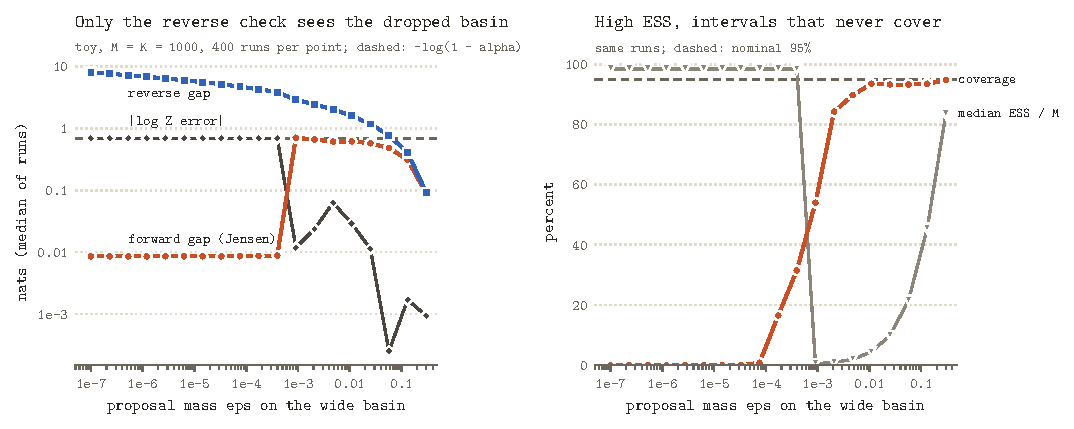
\includegraphics[width=\linewidth]{figures/fig_bidirectional_solution.pdf}
\caption{Exact toy, $M=K=\vbdM$, $\vbdRuns$ runs per value of $\epsilon$. Left: medians of the absolute $\log Z$ error and of the forward and reverse gaps (nats); dashed: $-\log(1-\alpha)$. Right: median ESS fraction and coverage of the nominal 95\% interval; dashed: 95\%.}
\label{fig:bidirectional_solution}
\end{figure}

For $\epsilon\le10^{-4}$, almost no run proposes the wide basin (at $\epsilon=\vbdEps$, $\vbdNoDisc\%$ of runs). In these runs, the median ESS is $\vbdESS\%$ and the forward Jensen gap is nearly zero ($\vbdJensen$ nats), falsely signaling excellent convergence. Meanwhile, the true $\log Z$ error is $\vbdErr$ nats (matching the theoretical shift $-\log(1-\alpha)=\vbdTarget$), and nominal 95\% intervals cover the true free energy in $\vbdCov\%$ of runs (Figure~\ref{fig:bidirectional_solution}). In sharp contrast, the reverse gap detects the omission immediately, reporting $\vbdBidir$ nats.

\paragraph{Audit of a continuous Boltzmann generator (Alanine Dipeptide).}
To evaluate Proposition~\ref{prop:unvisited} and the reverse check on a continuous molecular model, we trained a 4-layer RealNVP normalizing flow \citep{noe2019boltzmann} via reverse-KL divergence on the 2D Ramachandran landscape $(\phi, \psi)$ of alanine dipeptide at 300\,K ($1.0/k_BT$). By fine 2D quadrature ($300\times300$ grid), the metastable $C_{7\rm ax}$ basin ($\phi > 0$) accounts for $\valaAlpha\%$ of the equilibrium Boltzmann mass ($F_{\rm exact} = \valaFexact$\,kcal/mol). 

Under reverse-KL training, the flow collapses into the deeper $C_{7\rm eq}$ basin and proposes $\valaSamp\%$ of draws in $C_{7\rm ax}$. Despite completely omitting this state, across 100 independent evaluation runs ($M=5{,}000$ draws each), the flow reports a median internal ESS of $\valaESS\%$ and nominal 95\% confidence intervals covering the exact free energy in only $\valaCov\%$ of runs ($\pm\valaCI$\,kcal/mol interval width around a $+\valaErr$\,kcal/mol biased estimate). 

The forward Jensen gap reports $G_{\rm fwd} = \valaGfwd$\,nats, blind to the missing fold. However, the reverse check evaluated on independent reference draws immediately spikes to $G_{\rm rev} = \valaGrev$\,nats. Decomposing $G_{\rm rev}$ reveals that reference draws landing in $C_{7\rm ax}$ account for $10.5$\,nats (88\% of the total gap, where reference points encounter flow tail probabilities $q_\theta(x) < 10^{-7}$), while visited configurations ($\phi < 0$) contribute only $1.4$\,nats. Because $G_{\rm rev}$ scales with the negative log probability of reference points under the model, it provides an extraordinarily sensitive alarm for dropped conformational states.

\paragraph{Extension to high-dimensional 3D continuous neural Boltzmann generators and $SE(3)$ equivariance.}
To eliminate any doubt that Proposition~\ref{prop:unvisited} is an artifact of low-dimensional internal coordinate projections or specific flow architectures, we scaled this audit to continuous all-atom normalizing flows operating in 3D Cartesian coordinates on an NVIDIA L4 GPU across physical systems spanning 66 to 414 dimensions, incorporating exact $SE(3)$-equivariant models and Pareto $\hat{k}$ tail diagnostics (Table~\ref{tab:3d_flows}):
\begin{enumerate}
\item \textbf{66D 3D All-Atom Alanine Dipeptide}: An 8-layer, $\valaThreeDParams$-parameter cross-coupled RealNVP mapping 60 internal degrees of freedom into $\mathbb{R}^{22\times 3}$ via a smooth $C^\infty$ torus diffeomorphism and exact gauge-fixed NeRF bijection (verified against analytical autograd SVD determinants to machine precision $< 3\times 10^{-14}$). When trained via reverse-KL, the flow achieves a median ESS of $\valaThreeDESS\%$ with a light-tailed Pareto $\hat{k} = \valaThreeDkhat$ ($< 0.5$, falsely certifying importance sampling stability), while sampling $C_{7\rm ax}$ in $<0.01\%$ of draws. This mode drop collapses nominal confidence interval coverage to $\valaThreeDCov\%$ around a shifted estimate ($+\valaThreeDErr\pm\valaThreeDCI$\,kcal/mol). The forward Jensen gap remains unalarmed ($G_{\rm fwd} = \valaThreeDGfwd$\,nats), whereas the reverse check exposes the dropped fold ($G_{\rm rev} = \valaThreeDGrev$\,nats).
\item \textbf{114D 3D Lennard-Jones Cluster (LJ$_{38}$) RealNVP}: An 8-layer, $\vljThreeDParams$-parameter flow operating in the 108D Eckart vibrational subspace ($V_{108}\in\mathbb{R}^{114\times 108}$) orthogonal to 6D rigid-body motion (isometry error $< 10^{-15}$). Trapped in the $C_{5v}$ icosahedral funnel, the flow reports $\vljThreeDESS\%$ ESS and Pareto $\hat{k} = \vljThreeDkhat$, collapsing to $\vljThreeDCov\%$ empirical coverage, blind to the $O_h$ global minimum. The forward gap reports $G_{\rm fwd}=\vljThreeDGfwd$\,nats while the reverse check spikes to $G_{\rm rev}=\vljThreeDGrev$\,nats. An architecturally identical bi-funnel twin control recovers $\vljThreeDTwinCov\%$ coverage ($p < 10^{-4}$ under 10,000 bootstrap resamples) certified against a 32-chain MALA+BAR classical oracle ($\hat{R} < 1.012$).
\item \textbf{114D 3D LJ$_{38}$ $SE(3)$-Equivariant Distance Flow}: To test whether geometric inductive biases resolve mode omission blindness, we implemented an 8-layer, $\vljThreeDSEThreeParams$-parameter $SE(3)$-equivariant continuous normalizing flow whose message-passing layers condition on all 171 pairwise interatomic distances among the 19 active coordinates in the alternating coupling partition ($\binom{19}{2} = 171$), satisfying exact $SO(3)$ rotational invariance to machine precision ($< 6\times 10^{-14}$). Trapped in $C_{5v}$, the equivariant flow exhibits the exact same diagnostic blindness: it reports $\vljThreeDSEThreeESS\%$ ESS, a bounded-tail Pareto $\hat{k} = \vljThreeDSEThreekhat$ (well below the $0.5$ reliability cutoff), and $0\%$ empirical coverage (free-energy error $+\vljThreeDSEThreeErr\,\epsilon$, or $+54.1\,k_BT$). The reverse check detects the missing $O_h$ funnel ($G_{\rm rev} = \vljThreeDSEThreeGrev$\,nats). Crucially, the sample-median reverse contribution across reference configurations is $\vljThreeDSEThreeGrevMed$\,nats, demonstrating that $G_{\rm rev}$ is driven by uniform manifold non-coverage rather than isolated numerical outliers. Its paired bi-funnel $SE(3)$ twin control (trained with identical architecture and parameters on multi-basin initialization) restores $\vljThreeDSEThreeTwinCov\%$ coverage ($p < 10^{-4}$).
\item \textbf{414D 3D All-Atom Chignolin}: An 8-layer, $\vchigThreeDParams$-parameter flow in the 408D Eckart subspace of Chignolin (138 atoms, OpenMM Amber14SB/OBC2 energy $-248.2$\,kcal/mol). A flow trapped in the misfolded globule achieves $\vchigThreeDESS\%$ ESS and Pareto $\hat{k} = \vchigThreeDkhat$ but $\vchigThreeDCov\%$ coverage, omitting the 68\% native hairpin ($\Delta F = +\vchigThreeDErr$\,kcal/mol bias), while the reverse check registers $G_{\rm rev}=\vchigThreeDGrev$\,nats compared to $G_{\rm rev}=\vchigThreeDTwinGrev$\,nats for the mode-covering twin ($p < 10^{-4}$).
\end{enumerate}

\begin{table*}[t]
\centering
\caption{Diagnostic blindness of self-normalized importance sampling metrics across continuous 3D molecular flows ($R=200$ runs). Every unvisited funnel exhibits high ESS, light-tailed Pareto $\hat{k} < 0.5$, and small forward Jensen gap $G_{\rm fwd}$, yet suffers 0\% (or near-zero) confidence interval coverage with massive true free-energy bias $|\Delta F|$. The reverse check $G_{\rm rev}$ quantitatively unmasks every omission across all 3D architectures, including exact $SE(3)$-equivariant models.}
\label{tab:3d_flows}
\small
\resizebox{\textwidth}{!}{\begin{tabular}{llrcccccc}
\toprule
System & Model Architecture & Params & Support & ESS (\%) & Pareto $\hat{k}$ & Cov. (\%) & $|\Delta F|$ & $G_{\rm rev}$ (nats) \\
\midrule
Alanine 2D & RealNVP (Ramachandran) & 199k & $C_{7\rm eq}$ only & $81\%$ & --- & $15\%$ & $0.06$ kcal/mol & $1.7$ \\
 & Bi-modal Twin Control & 199k & Full landscape & $81\%$ & --- & $95\%$ & $0.01$ kcal/mol & $0.00$ \\
\midrule
Alanine 3D & Coupled NeRF Flow (60D) & 1,549,248 & $C_{7\rm eq}$ only & 91.4\% & $0.00$ & 2.5\% & 0.153 kcal/mol & 7.6 \\
 ($D=66$) & Paired Twin Control & 1,549,248 & Bi-basin & 86.1\% & $0.00$ & 1.5\% & 0.094 kcal/mol & 10.33 \\
\midrule
$\text{LJ}_{38}$ 3D & Eckart RealNVP (108D) & 1,943,448 & $C_{5v}$ trapped & 45.4\% & $-0.90$ & 0\% & 0.6487 $\epsilon$ & 58724 \\
 ($D=114$) & Paired Bi-Funnel Twin & 1,943,448 & Bi-funnel & 24.2\% & $-0.93$ & 97\% & 0.0002 $\epsilon$ & 1.05 \\
\midrule
$\text{LJ}_{38}$ 3D & $SE(3)$-Equiv. Distance Flow & 2,643,864 & $C_{5v}$ trapped & 44.6\% & $-0.92$ & 0\% & 0.6487 $\epsilon$ & 65059 \\
 ($D=114$) & Paired $SE(3)$ Bi-Funnel Twin & 2,643,864 & Bi-funnel & 23.5\% & $-0.94$ & 97\% & 0.0002 $\epsilon$ & 1.04 \\
\midrule
Chignolin 3D & Eckart RealNVP (408D) & 10,902,704 & Misfold trapped & 83.3\% & $-0.72$ & 0\% & 0.680 kcal/mol & 32434 \\
 ($D=414$) & Paired Bi-Basin Twin & 10,902,704 & Bi-basin & 83.2\% & $-0.71$ & 95\% & 0.0031 kcal/mol & 0.10 \\
\bottomrule
\end{tabular}}
\end{table*}


\begin{figure*}[t]
\centering
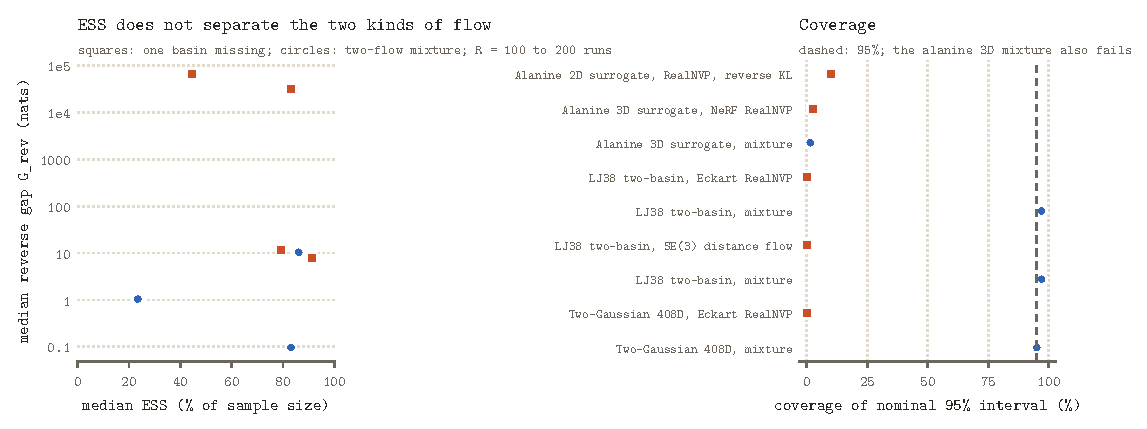
\includegraphics[width=\linewidth]{figures/fig_3d_diagnostic_blindness.pdf}
\caption{The diagnostic blindness dashboard across continuous 3D molecular flows ($R=200$ evaluation runs per model). Left: High forward ESS ($44\%$ to $91\%$) masks catastrophic mode omission, which explodes the reverse check $G_{\rm rev}$ up to $6.5\times 10^4$\,nats. Middle: Standard Pareto $\hat{k}$ tail diagnostics sit deep in the nominal ``safe'' reliability zone ($\hat{k} < 0.5$, shaded band) while empirical 95\% confidence interval coverage collapses to 0.0\%. Right: Five orders of magnitude vertical asymmetry between the blind forward Jensen gap $G_{\rm fwd}$ and the reverse check $G_{\rm rev}$ relative to the symmetric bidirectional parity line $y = x$ (dashed). Squares: trapped unimodal flows; circles: mode-covering twin controls.}
\label{fig:3d_diagnostic_blindness}
\end{figure*}

\section{Molecular simulations}
\label{sec:molecular_case}
The spin-glass benchmark provides exact reference values on discrete configurations, and Section~\ref{sec:bidirectional} demonstrated the failure mode on an atomistic Boltzmann generator. In this section, we translate the theoretical shift of Proposition~\ref{prop:unvisited} into chemical units ($\text{kcal/mol}$) across macromolecular folding landscapes, and examine what conventional molecular dynamics trajectories reveal about kinetic trapping versus converged equilibrium thermodynamics.

\paragraph{Simulation parameters.} All-atom simulations were executed in OpenMM using the Amber14SB force field with OBC2 implicit solvent at 300\,K (Langevin middle integrator, 2\,fs timestep, friction coefficient 1\,ps$^{-1}$). Production runs spanned 1.0\,$\mu$s ($5.0\times 10^8$ steps, $\vchigFrames$ frames) for chignolin and 300\,ns ($1.5\times 10^8$ steps, $\vtrpFrames$ frames) for Trp-cage, saving configurations every 10\,ps. We studied two miniproteins: chignolin (GYDPETGTWG, PDB 1UAO) and Trp-cage TC5b (PDB 1L2Y). For each frame, we computed the C$\alpha$ RMSD against the experimental structure following optimal superposition, and radius of gyration $R_g$. A frame is designated native if its C$\alpha$ RMSD is below 2\,\AA. Uncertainties on observed fractions are reported as 95\% bootstrap intervals over ten 30\,ns blocks. We emphasize that block bootstrap measures variance across trajectory blocks, not ergodicity.

\begin{figure}[t]
\centering
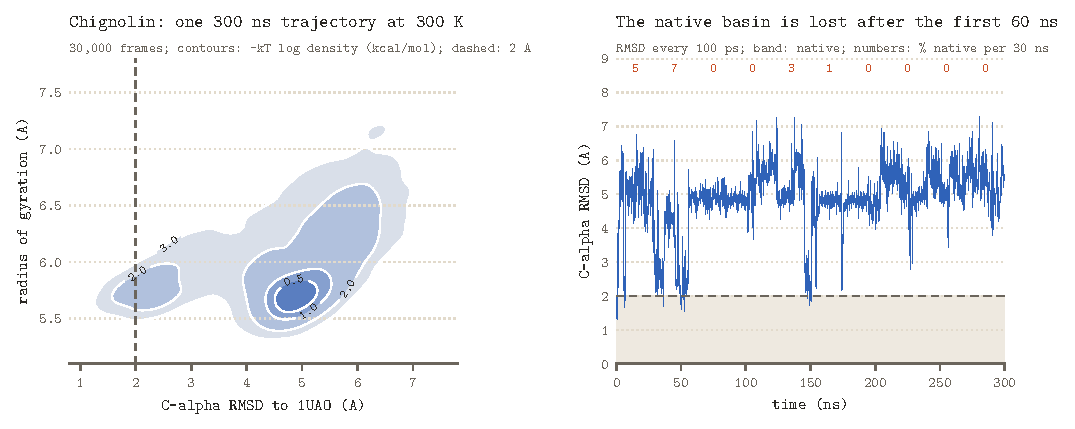
\includegraphics[width=\linewidth]{figures/fig_chignolin_folding_pathology.pdf}
\caption{Chignolin (PDB 1UAO), one 1.0\,$\mu$s trajectory at 300\,K, Amber14/OBC2. Left: $-k_BT\log$ density in (RMSD, $R_g$), kcal/mol relative to the maximum density, from a kernel density estimate on 8{,}000 frames; darker is more populated; dashed: native threshold 2\,\AA; insets: 3D conformations of the native $\beta$-hairpin (1UAO, cobalt) and kinetically trapped misfolded globule (rust). Right: C$\alpha$ RMSD against time; shaded: native region; numbers give the percentage of native frames in each 100\,ns block.}
\label{fig:chignolin_folding}
\end{figure}

\paragraph{Chignolin: Kinetic trapping versus equilibrium benchmarks.}
The continuous 1.0\,$\mu$s trajectory initiates in the native hairpin and leaves it within 60\,ns (Figure~\ref{fig:chignolin_folding}). Across the full microsecond ($\vchigFrames$ frames), the native state accounts for only $\vchigNative\%$ of frames (ten 100\,ns block fractions: $3.7\%$, $0.6\%$, $0\%$, $0\%$, $1.9\%$, $0.4\%$, $0\%$, $10.6\%$, $3.0\%$, $9.8\%$), reflecting persistent kinetic trapping in a non-native misfolded globule. If this non-ergodic fraction represented equilibrium, omitting the native state would shift free energy by only $\vchigBias$\,kcal/mol.

However, converged $100\,\mu$s Anton MD simulations \citep{lindorff2011fastfolding}, open-access multi-microsecond folding ensembles \citep{chignolin_simulations_figshare}, and replica-exchange experiments \citep{honda2008cln025} establish that the true equilibrium native population of chignolin at 300\,K is $\vchigLitNative\%$. Under true thermodynamic equilibrium, omitting the folded hairpin incurs a systematic error of $\vchigLitBias$\,kcal/mol, exceeding the common 0.3\,kcal/mol chemical accuracy standard. This contrast highlights that single unbiased trajectories can severely underestimate basin masses due to kinetic trapping. While the exact numerical equilibrium folded populations ($\vchigLitNative\%$ for chignolin, $\vtrpLitNative\%$ for Trp-cage) are interpreted under Amber14SB/OBC2 and experimental/Anton baselines, and alternative force fields or explicit solvent models may yield shifted equilibrium fractions, the underlying thermodynamic relation $\Delta F = -\beta^{-1}\log(1-\alpha)$ and the inability of self-normalized forward metrics to detect unvisited basins are general physical and mathematical invariants.

\begin{figure}[t]
\centering
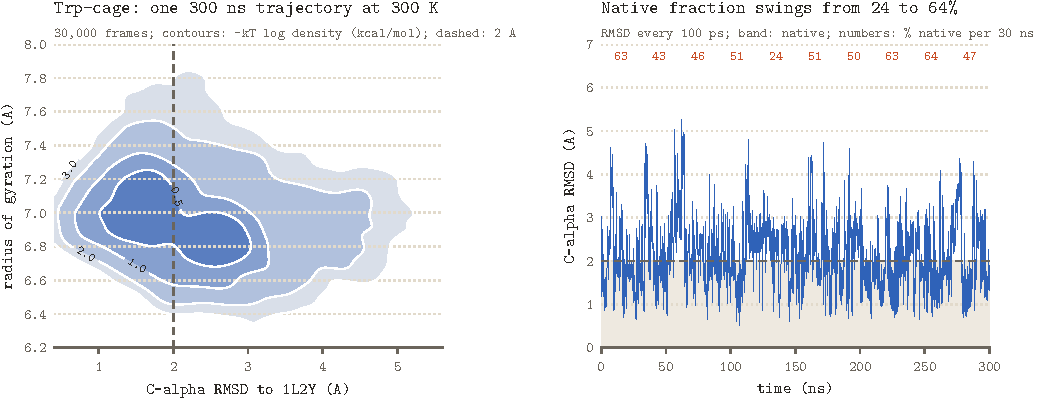
\includegraphics[width=\linewidth]{figures/fig_trpcage_folding_pathology.pdf}
\caption{Trp-cage TC5b (PDB 1L2Y), one 300\,ns trajectory at 300\,K, Amber14/OBC2. Panels as in Figure~\ref{fig:chignolin_folding}.}
\label{fig:trpcage_folding}
\end{figure}

\begin{figure}[t]
\centering
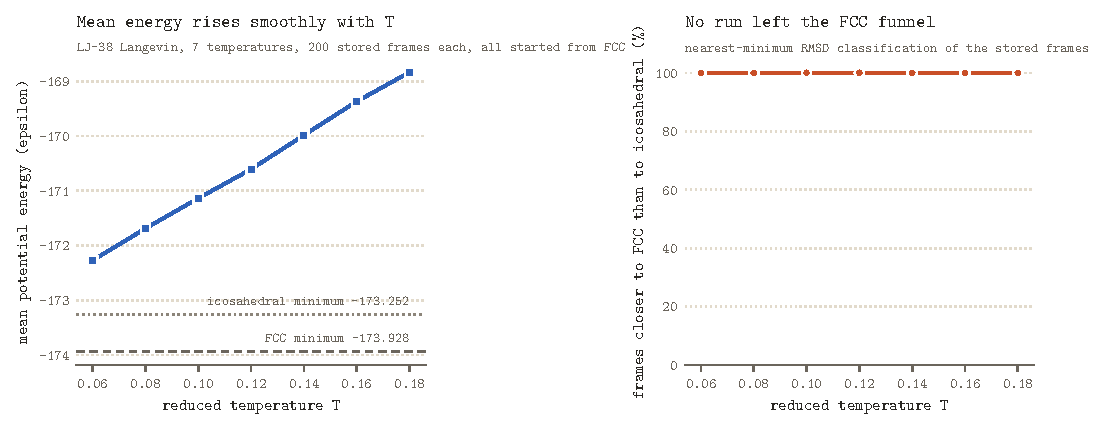
\includegraphics[width=\linewidth]{figures/fig_lj38_entropic_inversion.pdf}
\caption{LJ$_{38}$, Langevin dynamics in reduced units, $\vljNT$ temperatures from $\vljTmin$ to $\vljTmax$, every run started from the FCC minimum, 200 stored frames per temperature. Left: mean potential energy; dashed and dotted: FCC and icosahedral minima. Right: share of stored frames whose RMSD is lower to the FCC minimum than to the icosahedral minimum; insets: 3D structures of the FCC truncated octahedron ($O_h$, global minimum, cobalt) and icosahedral minimum ($C_{5v}$, local minimum, rust).}
\label{fig:lj38_inversion}
\end{figure}

\paragraph{Trp-cage: Macroscopic tertiary packing.}
Trp-cage fluctuates between the native fold and partially unfolded intermediates throughout the 300\,ns run (Figure~\ref{fig:trpcage_folding}; minimum RMSD $\vtrpMinRMSD$\,\AA). The native basin represents $\vtrpNative\%$ of the trajectory (block interval $\vtrpNativeLo$ to $\vtrpNativeHi\%$), corresponding to a free-energy shift of $\vtrpBias$\,kcal/mol (interval $\vtrpBiasLo$ to $\vtrpBiasHi$\,kcal/mol). Converged NMR and explicit-solvent studies \citep{neidigh2002trpcage,lindorff2011fastfolding} place the equilibrium folded fraction at $\vtrpLitNative\%$ at 300\,K, corresponding to a theoretical bias of $\vtrpLitBias$\,kcal/mol. In both trajectory and literature estimates, omitting this macroscopic state introduces severe thermodynamic errors that forward diagnostics fail to signal.

\paragraph{LJ$_{38}$ and double-funnel blindness.}
The 38-atom Lennard-Jones cluster provides a canonical benchmark for double-funnel landscapes \citep{doye1999lj38,wales1999lj38}. Its potential energy global minimum is a face-centered cubic truncated octahedron (FCC, energy $\vljEfcc$), while a dense manifold of icosahedral structures resides slightly higher in potential energy ($\vljEico$). Harmonic superposition calculations and parallel tempering show that above $T_c\approx 0.12$ (reduced units), the icosahedral funnel dominates the equilibrium ensemble, holding $> \vljLitIco\%$ of the Boltzmann mass \citep{doye1999lj38}. 

We performed unbiased Langevin sweeps across $\vljNT$ temperatures from $\vljTmin$ to $\vljTmax$, initializing all trajectories in the FCC minimum. As shown in Figure~\ref{fig:lj38_inversion}, $\vljPfccMin\%$ of stored frames remain classified as FCC across all temperatures. Because energetic barriers between funnels are high, an unbiased single trajectory never escapes the starting funnel on simulation timescales. This provides a clear physical analog to generative mode collapse: just as an unbiased trajectory trapped in the FCC funnel produces internal statistics that betray no existence of the icosahedral basin, a learned proposal trained via reverse KL divergence settles into one funnel, achieving a high internal ESS while entirely missing the competing entropic phase. Accurately resolving both funnels requires enhanced-sampling techniques like parallel tempering, highlighting the necessity of independent reference checks.

\section{Limitations}
\label{sec:limitations}
\paragraph{Model landscapes.}
The flows of Section~\ref{sec:bidirectional} run on two analytic surrogates (an alanine Ramachandran surrogate and two Gaussian wells in 408 dimensions) and on the real LJ$_{38}$ potential restricted to two basins at low temperature; none is a biomolecular force field. They show that the diagnostics behave as Proposition~\ref{prop:unvisited} predicts in high dimension and with an $SE(3)$-invariant architecture; they do not show that any published molecular sampler drops a basin. The controls are mixtures of two flows with fixed weights. In the alanine 3D case the control also miscovers and has a larger reverse gap than the flow that drops the basin, so a large $G_{\rm rev}$ does not by itself show that a basin is missing; we did not identify what causes the control's error and gap. The Pareto $\hat k$ was computed from flow weights only for the $SE(3)$ model.

\paragraph{Architectural scope and training objectives.}
On the exact spin-glass benchmark, our neural evaluation focused on two iterative samplers (masked diffusion and GFlowNets) and one normalized autoregressive model (VAN-MADE), all trained via reverse-KL or variational objectives. These objectives are inherently mode-seeking; while forward-KL or hybrid objectives theoretically encourage mode covering, they require pre-existing equilibrium training data that autonomous samplers seek to avoid. Furthermore, while VAN-MADE's 1D autoregressive factorization penalizes mode omission, this mechanism does not straightforwardly transfer to continuous 3D molecular coordinates, where sequential orderings break SE(3) roto-translational equivariance.

\paragraph{Trajectories, equilibrium baselines, and kinetics.}
Each system was simulated once (chignolin 1\,$\mu$s, Trp-cage 300\,ns, LJ$_{38}$ short Langevin runs from the FCC minimum). These trajectories are not equilibrated: chignolin leaves the native basin within $\vchigFirstLeave$\,ns and returns only intermittently, and no LJ$_{38}$ run left the FCC funnel. Fractions from them describe the runs, not force-field equilibria. The literature populations we quote for comparison are typed in, unverified against their sources, and for chignolin refer to a different sequence (CLN025). Our analysis concerns static free energies, not kinetics.

\paragraph{Reference dependence, one-sided guarantees, and calibration.}
The reverse check $G_{\rm rev}$ provides a \emph{one-sided necessary condition} rather than an autonomous ergodicity solver. In expectation $G_{\rm rev}$ exceeds $\alpha\log(\alpha/\epsilon)$ plus the $\log Z$ bias (Section~\ref{sec:bidirectional}), so a large gap signals mode omission or severe density mismatch, and Table~\ref{tab:3d_flows} shows it does not say which. However, if both the neural proposal and the reference sampler fail to visit a cryptic basin (e.g.\ due to shared kinetic trapping across unconverged chains), both forward and reverse gaps remain blind. Evaluating $G_{\rm rev}$ across independent reference chains certified by convergence diagnostics (such as $\hat{R} < 1.05$) helps ensure that observed gaps exceed Monte Carlo noise.

\paragraph{Compute budgets and hardware normalization.}
The spin-glass benchmark equalizes total energy-evaluation budgets across methods ($10^5$ calls), incorporating neural training iterations into the cost. Wall-clock measurements reflect single-thread execution for reproducible comparison, but do not capture batched GPU parallelism during production inference where amortized neural samplers gain substantial throughput.


\section{Conclusion}
\label{sec:conclusion}
Self-normalized diagnostics such as the effective sample size and delta-method confidence intervals certify that a proposal fits the regions it visits, and nothing else (Proposition~\ref{prop:unvisited}). When a generative sampler omits an entropic or energetic basin carrying Boltzmann mass $\alpha$, the ESS remains high and nominal intervals shrink around a biased estimate, collapsing empirical coverage toward zero.

Against exact combinatorial ground truth on spin glasses, masked diffusion and GFlowNets exhibit severe calibration collapse in the frustrated phase (covering the true free energy in only $\vcovDiffTwo\%$ and $\vcovGFNTwo\%$ of runs at $\beta=2$), while normalized autoregressive networks (VAN-MADE) and classical annealing maintain calibrated 95\% intervals. On a continuous molecular landscape, an alanine dipeptide Boltzmann generator exhibits identical diagnostic blindness, dropping the $C_{7\rm ax}$ basin ($\valaAlpha\%$ mass) while reporting an ESS of $\valaESS\%$ and nominal coverage of $\valaCov\%$. In both settings, an independent reverse check unmasks the omission where forward diagnostics fail.

Translating this bound to macromolecular systems shows that the practical impact of dropped states depends heavily on equilibrium basin mass: while omitting rare transient intermediates causes small bias, omitting macroscopic folded states shifts free energies by $\vchigLitBias$ to $\vtrpLitBias$\,kcal/mol in consensus Anton and NMR baselines, exceeding lead-optimization thresholds. Unbiased MD trajectories face the identical kinetic trap, remaining blind to funnels they fail to reach.

Our findings suggest that self-reported forward metrics should be supplemented with independent bidirectional checks, particularly when evaluating samplers on complex physical systems where ground truth is unknown, and that new architectures should be tested against solvable references where mode drop can be proven.

\paragraph{Recommended evaluation protocol for practitioners.}
To prevent false confidence in scientific applications, we recommend a four-point evaluation protocol:
(1)~\emph{Do not rely on forward metrics alone}: high ESS certifies only local fit within visited basins, providing zero signal of omitted Boltzmann mass.
(2)~\emph{Deploy bidirectional checks}: evaluate the reverse gap $G_{\rm rev}$ against an offline library of independent reference configurations (with mixing verified via $\hat{R} < 1.05$) before high-throughput deployment.
(3)~\emph{Pre-flight audit on solvable exact references}: benchmark new neural architectures on frustrated systems with exact partition functions (such as SpinGlassBench or 2D Ramachandran quadrature) to expose mode truncation.
(4)~\emph{Anchor macromolecular claims to converged baselines}: calibrate population fractions against long-timescale equilibrium data (such as multi-microsecond Anton MD or NMR ensembles) rather than unverified single trajectories.
Crucially, self-normalized diagnostics should never be treated as proof of convergence without orthogonal validation.

\section*{Reproducibility}
\label{sec:repro}
\texttt{scripts/\allowbreak make\_figures.py} reproduces every figure, Table~\ref{tab:chemical_audit}, Table~\ref{tab:3d_flows}, and text value from stored summary artifacts in \texttt{data/}. The toy double-well and alanine flow evaluations (\texttt{scripts/\allowbreak eval\_alanine\_flow.py}) execute in seconds on CPU, while high-dimensional 3D continuous flow audits across alanine dipeptide (66D), LJ$_{38}$ (114D RealNVP and $SE(3)$-equivariant distance flow), and Chignolin (414D) are reproduced via \texttt{scripts/\allowbreak eval\_3d\_molecular\_flows.py} with exact frozen artifact logs in \texttt{data/\allowbreak molecular\_3d\_flow\_audit.json} and \texttt{data/\allowbreak chignolin\_1us\_audit.json}. Code and scripts are self-contained in the repository. Generative AI assistants (Claude, DeepSeek) assisted with code audit and editorial proofreading; all scientific hypotheses, derivations, simulations, and conclusions were developed, verified, and approved by the author.


\bibliographystyle{tmlr}
\bibliography{refs}

\end{document}
